\Askhsh{17354_SOLUTION}{1}
\begin{ylh}{1}
    \item [Διάφορα θέματα Γεωμετρίας]
\end{ylh}
\begin{wrapfigure}[18]{r}{7cm}
    \centering
    \begin{tikzpicture}[scale=0.9]
        % Define points using coordinates derived to match the visual representation
        \tkzDefPoint(0,4){D} % Delta
        \tkzDefPoint(2,0){E}
        \tkzDefPoint(6,0){Z}
        \tkzDefPoint(0,0){K} % K is projection of D on EZ (extension through E)
        \tkzDefPoint(2.8,-1.6){I} % I is projection of Z on line DE (extension through E)

        % Draw triangle sides (solid)
        \tkzDrawSegment[line width=1pt](D,E)
        \tkzDrawSegment[line width=1pt](D,Z)
        \tkzDrawSegment[line width=1pt](E,Z)

        % Draw altitudes and extensions (dashed)
        \tkzDrawSegment[dashed,line width=1pt](D,K)
        \tkzDrawSegment[dashed,line width=1pt](Z,I)
        % Draw the line containing D, E, I as an extended dashed line
        \tkzDrawSegment[dashed,line width=1pt](D,I) % Draw from D to I, it will naturally extend E
        
        % Right angle at K
        \tkzMarkRightAngle[size=0.3](D,K,E) % Angle D-K-E for perpendicular DK to EZ

        % Right angle at I
        \tkzMarkRightAngle[size=0.3](Z,I,E) % Angle Z-I-E for perpendicular ZI to line DEI

        % Draw points
        \tkzDrawPoints(D,E,Z,K,I)

        % Labels
        \tkzLabelPoint[above](D){$\Delta$}
        \tkzLabelPoint[below](E){E}
        \tkzLabelPoint[below](Z){Z}
        \tkzLabelPoint[below](K){K}
        \tkzLabelPoint[below left](I){I}
    \end{tikzpicture}
\end{wrapfigure}
\kefalaio{ΛΥΣΗ}
\begin{alist}
    \item[α)]
    \begin{rlist}
        \item Η προβολή της πλευράς $\Delta E$ στην πλευρά $EZ$ είναι το τμήμα $\textbf{KE}$
        \item Η προβολή της πλευράς $\Delta Z$ στην πλευρά $EZ$ είναι το τμήμα $\textbf{KZ}$
        \item Το τμήμα $\Delta I$ είναι η προβολή της πλευράς $\Delta Z$ στην πλευρά $\Delta E$
        \item Το τμήμα $EI$ είναι η προβολή της πλευράς $EZ$ στην πλευρά $\Delta E$
        \item $\Delta Z^2 = \Delta E^2 + \textbf{EZ}^2 + 2 \cdot \textbf{EZ} \cdot \textbf{KE}$
        \item $\textbf{EZ}^2 = \textbf{\Delta E}^2 + \Delta Z^2 - 2 \cdot \textbf{\Delta E} \cdot \textbf{\Delta I}$
    \end{rlist}
    \item[β)] Το τμήμα $\Delta I$ είναι η προβολή της πλευράς $\Delta Z$ στην πλευρά $\Delta E$.
    Η γωνία $E\hat{\Delta}Z$ είναι οξεία γιατί ανήκει στο ίδιο τρίγωνο με τη γωνία $\Delta\hat{E}Z$, η οποία είναι αμβλεία, αφού τα ύψη $ZI$ και $\Delta K$ που αντιστοιχούν στις πλευρές της $\Delta E$ και $EZ$ αντίστοιχα, βρίσκονται εκτός του τριγώνου. Επομένως, εφαρμόζουμε το θεώρημα οξείας γωνίας στο τρίγωνο $\Delta EZ$ για την πλευρά $EZ$ και έχουμε:
    \[ EZ^2 = \Delta E^2 + \Delta Z^2 - 2 \cdot \Delta E \cdot \Delta I \text{ ή } 16=4+25-2 \cdot 2 \cdot \Delta I \text{ ή } 4\Delta I=13 \text{ ή } \Delta I = \frac{13}{4}. \]
\end{alist}